\documentclass[tikz, border = 2pt, varwidth]{standalone}

%---------------------------------------------------------------------------%
% PACKAGES                                                                  %
%---------------------------------------------------------------------------%

%----- MATH
%---------------------------------------------------------------------------%
\usepackage{amsmath, amssymb}

%----- FIGURES
%---------------------------------------------------------------------------%
\usepackage{pgfplots}
\pgfplotsset{compat=1.13}

\begin{document}

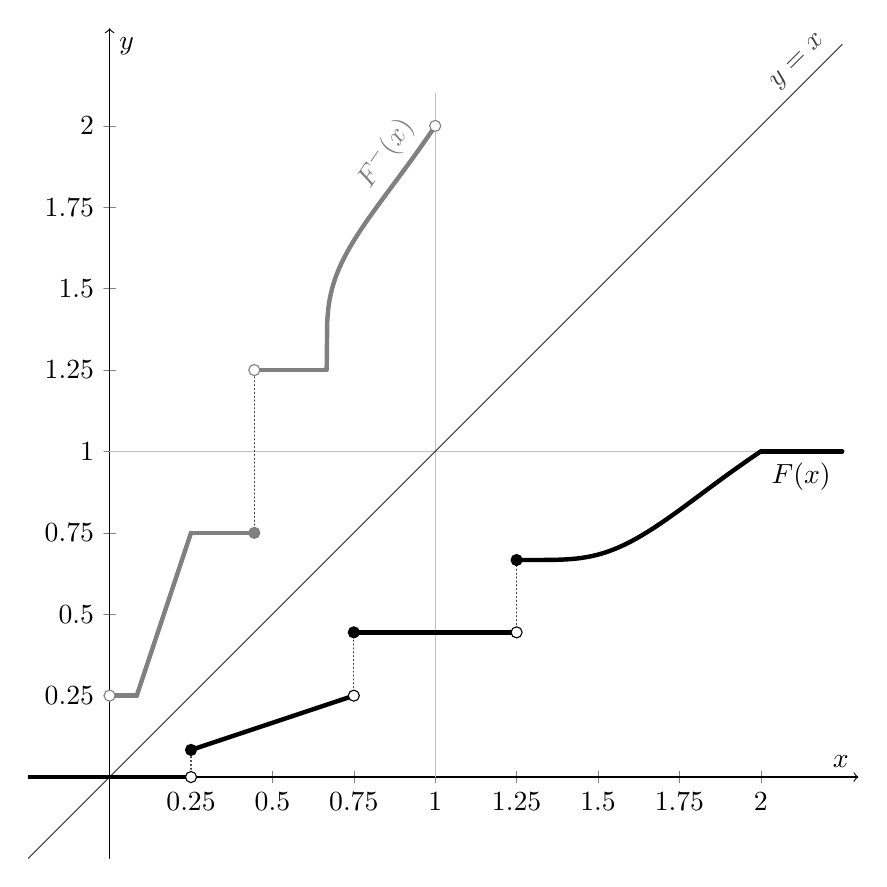
\begin{tikzpicture}
\begin{axis}[width = \textwidth,
height = \textwidth,
axis lines=middle,
inner axis line style={->},
xlabel={$x$},
ylabel={$y$},
ytick = {0,0.25,0.5,0.75,1,...,2},
xtick ={0,0.25,0.5,0.75,1,...,2},
legend pos = north east,
legend style = {draw=none},
legend cell align = left,
xmin = -.25,
xmax = 2.3,
ymin = -.25,
ymax= 2.3,
domain = -.5:2.25,
line cap = round
]
%
\addplot[mark = none, black!25, thin] coordinates {(0,1) (2.1,1)};
\addplot[mark = none, black!25, thin] coordinates {(1,0) (1,2.1)};
\addplot[mark = none, black!75, thin] {x} node[above, sloped, pos = 1, anchor =south east] {$y=x$};
%
\addplot[mark = none, black!75, thin, densely dotted] coordinates {(0.25,0) (0.25,1/12)};
\addplot[mark = none, black!75, thin, densely dotted] coordinates {(0.75,4/9) (0.75,3/12)};
\addplot[mark = none, black!75, thin, densely dotted] coordinates {(1.25,4/9) (1.25,{(exp(-16)+2)/3})};
%
\addplot[black, ultra thick, samples = 2, domain = -0.25:0.25] {0};
\addplot[black, ultra thick, samples = 2, domain = 0.25:0.75] {x/3};
\addplot[black, ultra thick, samples = 2, domain = 0.75:1.25] {4/9};
\addplot[black, ultra thick, samples = 200, domain = 1.25:2] {((exp(-1/(x-1)^2) - exp(-16))/(exp(-1)- exp(-16)) + 2)/3};
\addplot[black, ultra thick, samples = 2, domain = 2:2.25] {1} node[below, pos = 1, anchor =north east] {$F(x)$};
%
\addplot[only marks] coordinates {(0.25,1/12) (0.75,4/9) (1.25,{(exp(-16)+2)/3})};
\addplot[only marks, mark options = {thin, fill = white}] coordinates {(0.25,0) (0.75,3/12) (1.25,4/9)};
%%%
\addplot[mark = none, black!75, thin, densely dotted] coordinates {(4/9,0.75) (4/9,1.25)};
%
\addplot[black!50, ultra thick, samples = 2, domain = 0:1/12] {0.25};
\addplot[black!50, ultra thick, samples = 2, domain = 1/12:3/12] {3*x};
\addplot[black!50, ultra thick, samples = 2, domain = 3/12:4/9] {0.75};
\addplot[black!50, ultra thick, samples = 2, domain = 4/9:0.6666667] {1.25};
\addplot[black!50, ultra thick, samples = 200, domain = 0.6666667:1] {1+sqrt(-1/ln((exp(-1)-exp(-16))*(3*x-2)+exp(-16)))} node[below, pos = 1, sloped, anchor =south east] {$F^-(x)$};
%
\addplot[only marks, black!50] coordinates {(4/9,0.75)};
\addplot[only marks, black!50, mark options = {thin, fill = white}] coordinates {(0,0.25) (4/9,1.25) (1,2)};
%
\end{axis}
\end{tikzpicture}

\end{document}